\begin{figure}[!htbp]
    \centering
    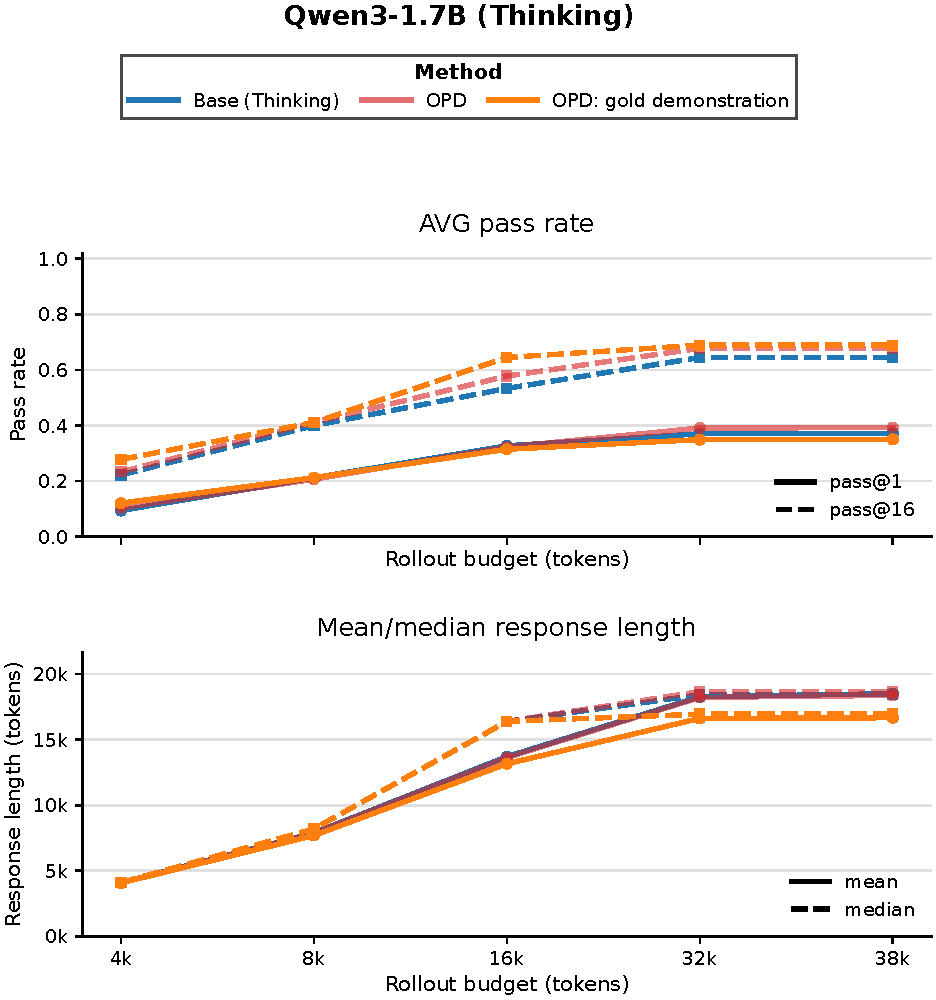
\includegraphics[width=\linewidth]{figures/avg_pass_rollout_tokens_qwen_1p7b_thinking_opd_gold_demo.pdf}
    \caption{
    \textbf{OPD with gold-demonstration context shortens response lengths while vanilla OPD preserves the base length profile.}
    This budget-curve companion to Table~\ref{tab:qwen17_openthoughts_opsd_opd} evaluates the \qwenonesevenb{} thinking student with a larger \qweneightb{} teacher.
    We compare the base model, vanilla OPD, and OPD with gold-demonstration teacher context.
    The OPD variants are trained with a 4,096-token completion cap, and all methods are evaluated at generation caps from 4,096 to 38,912 tokens.
    Top row: pass@1 and pass@16, averaged over AIME24, AIME25, and HMMT25.
    Bottom row: mean and median response length.
    Vanilla OPD mildly improves pass@k while largely preserving the base model's response-length curve.
    Adding gold-demonstration context to the teacher shortens responses and reduces the pass@1 gains; its long-budget degradation is milder than in the \opsd{} setting, consistent with the use of a stronger larger teacher.
    }
    \label{fig:qwen17_opd_gold_demo_budget_curves}
\end{figure}
